\chapter{Classification}

\section{Introduction}
Let's move from a regression setting to classification, also called decision making or hypothesis testing. In order to study classification, we will follow a path similar to the one on regression, that is we will find, at first, the best that we can do if we already have the model, then we will examine the case where the parameter is not random and finally we will study the supervised approach.

In classification, I have data $X$ and $\Theta$ that is the parameter I am interested in and it is discrete, which means that:
\[
    \Theta \in \{\theta_1, \theta_2, \dots, \theta_H\}
\]
where each $\theta_i$ is called a \textbf{class} or an \textbf{hypothesis}.

In some contexts, the parameter $\Theta$ is said to be \textbf{categorical}, which means that each class is a category. Since we are interested in the probability of each class, it's equivalent to consider them as a category or as a discrete number. However, there is a slight difference in the two terminologies, because if the parameter is discrete, then its classes will be numbers like $1, 2, \dots, H$, while if the parameter is categorical, then its classes will be categories such as cat, dog, bird, et cetera. For our purposes, it makes no differences.

In regression we quantify the error using as a metric the distance between the true value and the predicted value; thus it makes no sense to use categories in regression. In classification we don't care about the distance between categories, because the concept is not properly defined. We have only two possibilities that are: we belong to the category or not. Also, to quantify the error instead of using the MSE, we use the \textbf{probability of error}.

It is important to stress that in the classification problem, during the prediction we are not insterested in \textit{estimating} a class, but we are interested in \textit{make a choice} about the class.

\callout{Note}{There are no advantages in seeing the classification problem as a special case of a regression problem.}

We can formalize the error probability as:
\[
    \Pr{\hat{\Theta}(X) \neq \Theta }
\]

In telecommunication when the \textit{transmitter} sends a \textit{symbol}, the receiver has to decide which symbol has received among the finite number of possibilities. In that case, the optimal rule is the \textbf{maximum a posteriori probability (MAP)}. This rule is optimal when we have the likelihood function.

\section{Model-Based Classification}

\subsection{Bayesian approach}
Let us first use the bayesian approach to find the best performances. We define the \textbf{posterior distribution} of the hypothesis as the following p.m.f:
\[
    \Pr{\Theta = \theta \mid X}
\]
Also we define the \textbf{prior distribution} as the following p.m.f:
\[
    \pi(\theta) = \Pr{\Theta = \theta}
\]

Note that the most complete information about the parameter $\Theta$ is given by the posterior distribution. We cannot have more information than the one give by this distribution. Each other information can be derived from the posterior distribution.

Usually, the prior distribution is not very informative. Typically, if not specified, we assume that the prior distribution is uniform, which means that each class has the same probability to be the true class. This is a reasonable assumption when we have no information about the classes. In some cases, we can have some information about the classes, and in that case we can use a different prior distribution.
\[
    \pi(\theta_i) = \frac 1h\qquad i = 1, \dots, H
\]

In the continous case, it's more complex to give a shape to an uninformative prior distribution since the domain is infinitively large. However, there are some specifical distributions that are used as uninformative prior distributions.

It is intuitive and in this case correct to find that in order to minimize the probability of making a mistake, we decide for the parameter that has the highest probability according to the posterior distribution that has been obtained after visualizing the data, that is also the way to maximize the probability to make the right choice. Whatever other rule we use, we cannot have better results than the one obtained by using the posterior distribution.

\begin{figure}
    \centering
    \begin{minipage}{0.45\textwidth}
        \centering
        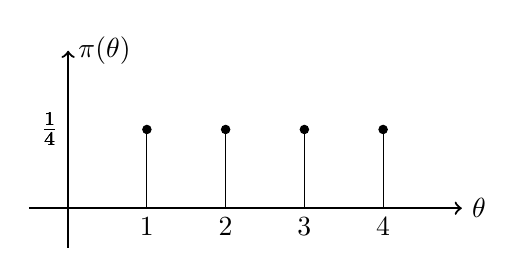
\begin{tikzpicture}[scale=1]
            % Axes
            \draw[->,thick] (-0.5,0) -- (5,0) node[right] {$\theta$};
            \draw[->,thick] (0,-0.5) -- (0,2) node[right] {$\pi(\theta)$};
            % Stem plot
            \foreach \x/\y in {1/1, 2/1, 3/1, 4/1} {
                    \draw (\x,0) -- (\x,\y);
                    \filldraw[black] (\x,\y) circle (1.5pt);
                    \node[below] at (\x,0) {\x};
                    \node[left] at (0,\y) {$\frac{1}{4}$};
                }
        \end{tikzpicture}
    \end{minipage}

    \vspace{1cm}

    \begin{minipage}{0.45\textwidth}
        \centering
        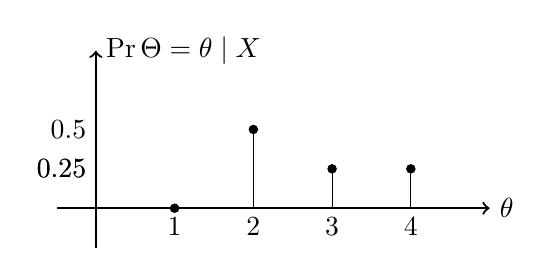
\begin{tikzpicture}[scale=1]
            % Axes
            \draw[->,thick] (-0.5,0) -- (5,0) node[right] {$\theta$};
            \draw[->,thick] (0,-0.5) -- (0,2) node[right] {$\Pr{\Theta = \theta \mid X}$};

            \draw (1,0) -- (1,0);
            \filldraw[black] (1,0) circle (1.5pt);
            \node[below] at (1,0) {1};

            % Stem plot
            \foreach \x/\y in {2/1, 3/0.5, 4/0.5} {
                    \draw (\x,0) -- (\x,\y);
                    \filldraw[black] (\x,\y) circle (1.5pt);
                    \node[below] at (\x,0) {\x};
                    \pgfmathsetmacro{\ytick}{\y/2}
                    \node[left] at (0,\y) {\ytick};
                }
        \end{tikzpicture}
    \end{minipage}

    \caption{Classification example}
    \label{fig:classificationexample}
\end{figure}

A typical situation is described in figure \ref{fig:classificationexample}, in which after visualizing the data we are able to find the posterior distribution and so the hypothesis that has the highest probability to be the true one.

\paragraph*{Bayes' update}
In this setting we're working with two quantities: the \textit{prior} distribution and the \textit{likelihood} function. The likelihood function is the generative mechanism of the data, while the prior distribution is the information we have about the classes before observing the data. These two quantities are connected to the posterior distribution by \textbf{Bayes' rule}.
Let's recall the Bayes' rule:
\[
    \mu(\theta \mid X) = \frac{\pi(\theta) \ell(X \mid \theta)}{\sum_{\theta'} \pi(\theta') \ell(X \mid \theta')} \propto \pi(\theta) \ell(X \mid \theta)
\]

This posterior function is also said to be the \textbf{belief} of the system. It is the probability that the true class is $\theta$ given the data $X$. Clearly, this function is a \textit{probability mass function}.
The process of finding the posterior distribution from the prior distribution and the likelihood function is called \textbf{Bayes' update}.

The denominator of the Bayes' rule is a normalizing constant that makes the posterior distribution a probability mass function. It is also called \textbf{marginal distribution}.
When $X$ is frozen, the marginal distribution is just a normalizing constant, so the belief is proportional to prior times the likelihood.

\subsubsection*{Behavior on multiple data}
Assume that I observe $X = \left[X_1, \dots, X_n\right]$ that are i.i.d according to $\ell(X_i \mid \theta_0)$, where $\theta_0$ is one of our hypothesis and we know that it's the true one.
Ideally, I'd want that, if the true hypothesis is $\theta_0$, not only the probability of error is zero, that is:
\[
    P_{err} = \sum_{\theta_i}\pi(\theta_i)P[err\mid \theta_i] \to 0
\]
but also that the system has the highest posterior distribution possible. That is:
\[
    \lim_{n \to \infty} \mu(\theta_0 \mid X) = 1
\]

This is reasonable because, in a good learning system, if we have a lot of data, we should be able to find the true hypothesis with high probability.
The more the data, the more is the confidence into the given choice of the hypothesis.

\begin{proof}
    Let's consider the posterior distribution of interest:
    \[
        \mu(\theta_0 \mid X) = \frac{\pi(\theta_0) \prod_{i=1}^N \ell(X_i \mid \theta_0 )}{\sum_{\theta'} \pi(\theta') \prod_{i=1}^N \ell(X_i \mid \theta')}
    \]

    The denominator of the previous quantity is a disturbing term, so, we can consider the ratio between the posterior distribution of the true hypothesis $\theta_0$ and the posterior distribution if the parameter is a certain $\theta \neq \theta_0$ to cancel out the denominator:
    \[
        \frac{\mu(\theta_0 \mid X)}{\mu(\theta \mid X)} = \frac{\pi(\theta_0) \prod_{i=1}^N \ell(X_i \mid \theta_0 )}{m(x)} \frac{m(x)}{\pi(\theta) \prod_{i=1}^N \ell(X_i \mid \theta)} = \frac{\pi(\theta_0)}{\pi(\theta)} \frac{\prod_{i=1}^N \ell(X_i \mid \theta_0)}{\prod_{i=1}^N \ell(X_i \mid \theta)}
    \]

    Since we want to analyze an \textbf{asymptotic behaviour}, a useful result that match the condition is the \textbf{law of large numbers}. In order to apply it we need to move in the favorable condition of a sum of terms. To do that, we move in a logarithmic space, this operation is allowed because the logarithm is a monotonic function.
    By applying the log to both members:
    \[
        \log \left(\frac{\mu(\theta_0 \mid X)}{\mu(\theta \mid X)}\right) = \log \left(\frac{\pi(\theta_0)}{\pi(\theta)}\right) + \log\left(\frac{\prod_{i=1}^N \ell(X_i \mid \theta_0)}{\prod_{i=1}^N \ell(X_i \mid \theta)}\right)
    \]
    Observe that by applying logarithm property, the product becomes a sum. And, for the same reason followed before, we divide both members by $n$:
    \[
        \frac{1}{n} \log \left(\frac{\mu(\theta_0 \mid X)}{\mu(\theta \mid X)}\right) =\frac{1}{n} \log \left(\frac{\pi(\theta_0)}{\pi(\theta)}\right) + \frac{1}{n} \sum_{i=1}^N \log \left(\frac{\ell(X_i \mid \theta_0)}{ \ell(X_i \mid \theta)}\right)
    \]
    Let's now consider what happens when $n$ approaches infinity.
    \[
        \lim_{n \to \infty} \frac{1}{n} \log \left(\frac{\mu(\theta_0 \mid X)}{\mu(\theta \mid X)}\right) = \lim_{n \to \infty} \frac{1}{n} \log \left(\frac{\pi(\theta_0)}{\pi(\theta)}\right) + \lim_{n \to \infty} \frac{1}{n} \sum_{i=1}^N \log \left(\frac{\ell(X_i \mid \theta_0)}{ \ell(X_i \mid \theta)}\right)
    \]
    The first term in the second member goes to zero because the ratio of the priors is a finite number, ignoring eventually zero probability events because there is no point in considering them in a discrete context.
    While the second term converges (according to the law of large numbers) to an expected value \textbf{computed under the distribution of the true hypotesis} of the logarithm of the ratio of the likelihoods.

    \[
        \lim_{n\to\infty} \frac{1}{n} \log \left(\frac{\mu(\theta_0 \mid X)}{\mu(\theta \mid X)}\right) = \E{\ell(\cdot \mid \theta_0)}{\frac{\ell(X_i \mid \theta_0)}{ \ell(X_i \mid \theta)}}
    \]

    The expected value is computed under that distribution because we want to consider all theh possible values of the data $X_i$ that are generated, and they are generated according to the \textit{generative mechanism} dictated by the true hypothesis $\theta_0$.

\end{proof}

Note that there is a physical meaning when the ratio of the prior goes to $0$. This means that the prior information is ignored when we have a lot of data. This is a good property because it means that the system is learning from the data and not from the prior information. Moreover, this is useful beacause if we have a wrong or biased prior information, by considering a lot of data we're going to ignore it.

The final obtained expectation is called \textbf{Kullback-Leibler divergence} and it's a measure of the \textit{relative entropy}.
\[
    \E{\ell(\cdot \mid \theta_0)}{\frac{\ell(X_i \mid \theta_0)}{ \ell(X_i \mid \theta)}} \triangleq D_{KL} (\theta_0 \mid\mid \theta)
\]
In general, the Kullback-Leibler divergence explains how different are two distributions. It is a non-negative number that is zero if and only if the two distributions are equal. The greater the distributions are different, the greater the divergence.

If $p$ and $q$ are two pmfs, then:
\[
    D_{KL}(p \mid \mid q) =\sum_{x \in X} p(x) \log\frac{p(x)}{q(x)} = \E{p}{\log \frac{p(x)}{q(x)}}
\]

If $p$ and $q$ are two pdfs, then:
\[
    D_{KL}(p \mid \mid q) =\int p(x) \log\frac{p(x)}{q(x)} dx
\]

\callout{Warning}{It's incorrect to say that the Kullback-Leibler divergence is a distance. It is not symmetric.}

Now we're going to prove that, given that the ratio of belief converges to the Kullback-Leibler divergence, our system learns the correct hypothesis.

\begin{proof}
    We've shown that the quantity for $n \to +\infty$ converges to the Kullback-Leibler divergence. This quantity is a non-negative quantity and if we add the \textbf{identifiabilty} assumption we know that is a positive quantity.
    \[
        \frac{1}{N} \log\frac{\mu(\theta_0 \mid X)}{\mu(\theta \mid X)} \to D_{KL} (\theta_0 \mid \mid \theta) > 0
    \]
    \callout{Note}{For simplicity we're going to use the notation $D_{KL}(\theta_0 \mid \mid \theta)$ instead of $D_{KL}(\ell(\cdot \mid \theta_0) \mid \mid \ell(\cdot \mid \theta))$}
    The \textbf{identifiability} assumption is necessary since it tells that $\ell(x\mid \theta_0) \neq \ell(x \mid \theta)$. So we're assuming that no one of our hypothesis share the same model, otherwise it'd be possible to have a Kullback-Leibler divergence equal to zero.

    Observe that, if that quantity converges to a finite and positive number, if we remove the $\frac 1N$ ration by multiplying both members by N, we get that the first member goes to $+\infty$.
    A logarithm will diverge only if its argument diverges:
    \[
        \frac{\mu(\theta_0 \mid X)}{\mu(\theta \mid X)} \to +\infty
    \]
    This quantity can diverge either if:
    \begin{itemize}
        \item the numerator goes to infinity
        \item the denominator goes to zero
    \end{itemize}

    Since the posterior distribution at the numerator is a probability, it is a finite number, and the only possible event is that $\mu(\theta\mid X) \to 0 $. This implies, given the identifiability property that $\mu(\theta_0 \mid X) \to 1$.
\end{proof}


Now, we are going to find what happens if our data is generated by an arbitrary function $f$, that we are going to assume that no one of our hypothesis is the true one.

As in the previous proof, we are going to compute the ratio between the belief of $\theta$ given $x$ and the belief of a $\theta^{\prime}$ given $x$.
\[
    \frac{\mu(\theta \mid x)}{\mu(\theta^{\prime} \mid x)} = \frac{\pi(\theta) \ell(x \mid \theta)}{\pi(\theta^{\prime} \ell(x \mid \theta^{\prime} ))} = \frac{\pi(\theta)}{\pi(\theta^{\prime} )} \prod_{i=1}^N \frac{\ell(x_i \mid \theta)}{\ell(x_i \mid \theta^{\prime} )}
\]
Now we apply the logarithm to both members and we divide both members by $n$:
\[
    \frac{1}{n} \log \frac{\mu(\theta \mid x)}{\mu(\theta^{\prime} \mid x)} = \frac{1}{n} \log \frac{\pi(\theta)}{\pi(\theta^{\prime} )} +  \frac{1}{n} \sum_{i=1}^n \log \frac{\ell(x_i \mid \theta)}{\ell(x_i \mid \theta^{\prime} )}
\]

Let's define a new random variable: %TODO: mi sfugge la necessità di definire una nuova v.a.
\[
    Z_i = \log \frac{\ell(x_i \mid \theta)}{\ell(x_i \mid \theta^{\prime} )}
\]
Then we got:
\[
    \frac{1}{n} \log \frac{\mu(\theta \mid x)}{\mu(\theta^{\prime} \mid x)} = \frac{1}{n} \log \frac{\pi(\theta)}{\pi(\theta^{\prime} )} + \frac{1}{n} \sum_{i=1}^n Z_i
\]
where each $Z_i$ is independent and identically distributed to the ratio of the likelihoods. When $n$ goes to $+\infty$, according to the law of large numbers we know that the term on the right converges to the expected value of $Z$
\[
    \lim_{n\to\infty }\frac{1}{n} \log \frac{\mu(\theta \mid x)}{\mu(\theta^{\prime} \mid x)} = \E{}{Z} %TODO: credo sia errato -> \E{Z}{\log \frac{\ell(x \mid \theta)}{\ell(x \mid \theta^{\prime} )}}
\]
Each $Z_i$ is generated by the true generative mechanism that is the function $f(X)$. Thus we can write:
\[
    \frac{1}{n} \log \frac{\mu(\theta \mid x)}{\mu(\theta^{\prime} \mid x)} = \E{f}{\log \frac{\ell(x \mid \theta)}{\ell(x \mid \theta^{\prime} )}}
\]
It's easy to understand that in this case we're not converging to the Kullback-Leibler divergence, since we're not computing the expected value under the same distribution that is at the numerator of the logarithm.
However, we can try to manipulate the expression to find a relationship with the Kullback-Leibler divergence. Since we want to obtain divergences, we can insert the $f(X)$ into the expected value by multiplying and dividing the argument of the logarithm by $f(X)$.
And, after some manipulation, we can find that:
\[
    \E{f}{\log \frac{\ell(x \mid \theta)}{\ell(x \mid \theta^{\prime} )} \frac{f(X)}{f(X)}} = \E{f}{\log \frac{f(x)}{\ell(x \mid \theta^{\prime} )}} - \E{f}{\log\frac{f(x)}{\ell(x \mid \theta)}}
\]
So we've found that the expression can be written as the difference of two Kullback-Leibler divergences.
\[
    \lim_{n\to\infty }\frac{1}{n} \log \frac{\mu(\theta \mid x)}{\mu(\theta^{\prime} \mid x)} = D_{KL} \left(f || \ell(\cdot \mid \theta^{\prime} )\right) - D_{KL}\left(f || \ell(\cdot \mid \theta)\right)
\]
let's rewrite the this expression by using a slightly simplified notation:
\[
    \frac{1}{n} \log \frac{\mu(\theta \mid x)}{\mu(\theta^{\prime} \mid x)} \xrightarrow{n \to +\infty} D_{KL} \left(f || \theta^{\prime} \right) - D_{KL}\left(f ||  \theta\right)
\]
In order to find \textit{which hypothesis will the system learn}, we need to recall that the chain of implications in the previous proof, required the ratio of beliefs to converge to a positive value (when $n$ approaches $+\infty$):
\[
    \lim_{n\to\infty} \frac{1}{n} \frac{\mu(\theta^\ast \mid X)}{\mu(\theta^{\prime}  \mid X)} \to D_{KL} \left(f || \theta^{\prime} \right) - D_{KL}\left(f ||  \theta\right) > 0
\]
Now, we consider a $\theta^\ast$ that isn't an arbitrary hypothesis, but we assume there exists:
\[
    \theta^\ast \colon D_{KL}\left(f||\theta^{\prime} \right) > D_{KL} \left(f||\theta^\ast\right) \qquad \forall \theta^{\prime} \neq \theta^{\ast}
\]
If this condition is satisfied, then the chain of implications used in the last lecture holds again and we can use it to prove that $\mu(\theta^{\ast} \mid X) \to 1$.

\textbf{Note} that $\theta^{\ast} $ is the hypothesis that has the smalled distance (in terms of the Kullback-Leibler divergence) from the true distribution.

The hypothesis $\theta^\ast$ will surely exists because, since we have a finite number of hypothesis, we can find the one that has the smallest distance from the true distribution. This is a consequence of the fact that the Kullback-Leibler divergence is a non-negative quantity and it is zero if and only if the two distributions are equal but we assume that this can't happens.

\begin{figure}
    \centering
    \begin{tikzpicture}[scale=1.5]
        \def\truef#1{-exp(-3*(2*#1 - 1)^2) + 2*exp(-0.5*(2*#1 - 1)^2)}
        % Axes
        \draw[->,thick] (-3.7,0) -- (4,0) node[right] {$x$};
        \draw[->,thick] (0,-0.5) -- (0,2) node[above] {pdf};

        % Curve
        \draw[red,domain=-3.5:0.5,samples=100] plot (\x, {1.5*exp(-3*(\x + 2)^2)});

        \draw[black, dashed, domain=-1:2.5,samples=100] plot (\x, {\truef{\x}});

        \draw[yellow,domain=1:3.5,samples=100] plot (\x, {1.5*exp(-3*(\x - 2)^2)});

        \node[above] at (-2,1.5) {$\ell(x\mid \theta_1)$};
        \node[above] at (0.5, 1.5){true f};
        \node[above] at (2,1.5) {$\ell(x\mid \theta_2)$};
    \end{tikzpicture}
    \label{fig:klexample}
    \caption{Kullback-Leibler divergence example}
\end{figure}

In the example of figure \ref{fig:klexample}, we can see that the true distribution is the one in the middle.
The two other distributions are the likelihood functions of two different hypothesis. We can see that the hypothesis that has the smallest distance from the true distribution is the one on the right. In this particular case, the divergence is also the distance between the two distributions but is not general.
In this example, our system will learn the hypothesis $\theta_2$ because $\ell (x \mid \theta_2)$ is the one with the lowest divergence from the true distribution.

% From this proof, we found out that our model approximates the truth when our model is the closest in terms of Kullback-Leibler divergence to the true model.
So, given a certain distribution of the data $f$, the system will learn the hypothesis that is the closest to the true distribution in terms of Kullback-Leibler divergence.

Note that this is the general case, and the previous proof was a special case of this. It is simple to show that if $f(x) = \ell(x \mid \theta_0)$, the minimum will be the true hypothesis $\theta_0$.

This is an important result since it also tells us that if the system are using wrong models to update the belief, if that models are not so far from the true model, the system will learn the true model. This is a good property because it means that the system is robust to the model used to update the belief.

\paragraph*{On the Bayes' update}
Having defined
\[
    \mu_n(\theta) \triangleq \mu(\theta \mid x_1, \dots, x_n)
\]
We want to find a relationship between $\mu_n(\theta)$ and $\mu_{n-1}(\theta)$.
We know that:
\[
    \mu_n(\theta) \propto \pi(\theta) \prod_{i=1}^n \ell(x_i \mid \theta) = \pi(\theta) \prod_{i=1}^{n-1} \ell(x_i \mid \theta) \ell(x_n \mid \theta)
\]
and that
\[
    \mu_{n-1}(\theta) \propto \pi(\theta) \prod_{i=1}^{n-1} \ell(x_i \mid \theta)
\]
So we can infer that:
\[
    \mu_n(\theta) = \mu_{n-1}(\theta) \ell(x_n \mid \theta)
\]
This is none other that \textit{Bayes' rule} where our past belief $\mu_{n-1}(\theta)$ is the current prior. This property, called \textbf{sequential property}, explains why we talked about \textit{Bayes' updates}: by doing successive updates we starts from the prior and step by step we update our belief with new evidence given from the likelihood.

This property holds only thanks to the hypothesis of \textbf{independendence} of the data. With an independent model, all the knowledge we have at a certain step is contained in the current belief. This property is really important, due to computation reasons, because it simplifies the calculations and allows to use Bayes updates in a streaming setting. In some ways it can be considered as a form of online learning.

By the way, sometimes this approach is used also when the data is not independent because a lot of times we don't have any other choice.
\subsection{Neyman-Pearson Criterion}
Now we want to find what happens when our parameter $\Theta$ is deterministic. First of all, let us clarify that in the Bayes problem we encountered before, $\Theta$ was random, even though we worked with fixed value of theta. This is because the same reasoning applies to any choice of the hypothesis.

Suppose we have only $2$ classes, that are $\theta \in \{-1, 1\}$. In this case our perfromance metric is not simply the error probablity, because we have two different error probabilities:
\begin{gather*}
    \alpha = \Pr{\text{choose } 1 \mid -1\text{ is true}} \qquad \text{ type 1 error probability} \\
    \beta = \Pr{\text{choose } -1 \mid 1\text{ is true}} \qquad \text{ type 2 error probability}
\end{gather*}
In some contexts, $\alpha$ and $\beta$ are also called \textbf{false positive} and \textbf{false negative} probabilities. But for generality we will refer to them as type 1 and type 2 error probabilities.
\callout{Note}{It is important to stress that the only indicators we will need to explain classification are the ones contained in the ROC curve.}
By contrast, in the Bayesian setting, our error probability was given, according to the theorem of the total probability, by the weighted arithmetic average of the two errors:
\[
    P_{err} = \alpha \pi(-1) + \beta \pi(+1) = \alpha \pi(-1) + \beta [1-\pi(-1)]
\]

Now we want to find the optimal strategy to use in this setting. Note that we cannot minimize both errors, because if we lower one error, the other one increases.
In fact, a decision rule would compare a function of the data $g(X)$ to a threshold $\gamma$.
\[
    g(X) \lessgtr^{-1}_{+1} \gamma
\]

If we lower the threshold, we lower the type 1 error probability, but we increase the type 2 error probability. And vice versa.
So, we will have to find a trade off between the two errors.

The optimal strategy and the most adopted one is the \textbf{Neyman-Pearson Criterion}, which requires to \textbf{minimize $\beta$ over all possible strategies that ensure that $\alpha \leq \alpha^\ast$.}
The solution of this criterion is to compare the likelihood ratio to a threshold $\gamma$, which depends on $\alpha^\ast$:
\[
    \frac{\ell(x \mid +1)}{\ell(x \mid -1)} \lessgtr^{-1}_{+1} \gamma_{\alpha^\ast}
\]
This criterion supposes to can tollerate a certain type 1 error probability $\alpha^\ast$ and it minimizes the type 2 error probability by consequence. It can also be seen from the other side, that is, it supposes to can tollerate a certain type 2 error probability $\beta^\ast$ and it minimizes the type 1 error probability by consequence.

The relationship between the threshold and the type 1 error probability is inversely proportional, as we can also note from the \textbf{Receiver Operating Characteristic (ROC) curve} that describes the realtionship between $\alpha$ and $1-\beta$ when $\gamma$ varies.
A good ROC curve is a concave curve that is close to the top-left corner of the plot. The closer the curve is to the top-left corner, the better the classifier is.

\begin{figure}
    \centering
    \begin{tikzpicture}[scale=1.5]
        % Axis
        \draw[thick,->] (0,0) -- (4,0) node[anchor=north west] {$\alpha$};
        \draw[thick,->] (0,0) -- (0,4.5) node[anchor=south east] {$\beta$};
        \draw[thick, red, dashed] (0,0) -- (0,4) -- (4,4);
        % Curve
        \draw[blue] (0,0) to[out=90,in=180] (4,4);

        % Random classifier line
        \draw[dashed] (0,0) -- (4,4);
        % Labels
        \node[below left] at (0,0) {0};
        \node[below right] at (5,0) {1};
        \node[above left] at (0,4) {1};
        \node[below] at (2,0) {0.5};
        \node[left] at (0,2) {0.5};

    \end{tikzpicture}
    \caption{ROC curve}
    \label{fig:roc}
\end{figure}

The straight line in the ROC curve of figure \ref{fig:roc} is the silliest decisor, which uses a \textit{randomized rule}, for example, if $\alpha=0.5$ and $\beta=0.5$, it flips a coin and decides.
That situation can also be seen as the case in which, in order to increase the value of $1-\beta$, we have to increase the value of type 1 error probability $\alpha$. This is not a desirable behaviour.

\section{Supervised Classification}
In the previous sections, we have seen model-based classification, both the bayesian setting and the Neyman-Person case. Now, we will see how to perform supervised classification. The setting is similar to the one of the regression.
We have our classes
\[
    \Theta \in \{\theta_1, \theta_2, \dots, \theta_H\}
\]
and our features
\[
    X \in \mathbb{R}^d
\]
As in the regression case, we will have to define a risk function based on the model-based theory (the MMSE) and then use the empirical version of the risk to perform the supervised classification.

In the regression case, we have seen that the MMSE is
\[
    \text{MMSE} = \min_f \mathbb{E}\left[ \left( Y - f(X) \right)^2 \right]
\]
We haven't specified the shape of the function $f$, but it needs to be an integrable function.
However, when we need to let the calculator to solve the optimization problem we need to specify the shape of the function $f$ in order to derive the optimal parameter (and it's the same thing we do in deep learning).

So, as we've done in regression for the optimal regression function, we now replace the ideal classification object $\mu(\theta\mid X)$ with its empirical version $\hat{\mu}_\beta(\theta \mid X) \in \mathcal F$. $\mathcal F$ will be a parametric class, which has $\beta$ as a paramater.
The fundamental requirement is that $\hat \mu_{\beta}(\theta \mid X)$ will always be a probability mass function.

Coming back to the risk function. In the regression case, we used the mean square error. In the classification case, we can use the Kullback-Leibler divergence to measure the "distance" from the optimal object.
% Assume that now we have picked a model. Our goal is to find a function $\hat{\mu}$ which error probability is comparable to the one of $\mu$. But there is a problem that we have to replace the error probability with something that we can use in optimization theory. We can use the Kullback-Leibler divergence.

So now, given that we're estimating our ideal object $\mu(\theta\mid X)$ with $\hat\mu_{\beta}(\theta\mid X)$, our goal is to find the parameter $\beta$ that minimizes the Kullback-Leibler divergence between the two distributions:
\[
    \beta^\ast = \arg\min_{\beta \in \mathbb{R}^M} {D}_{KL}\left( \mu\mid\mid \hat{\mu}_\beta\right) % ho rimosso la bar per far evincere l'errore
\]

By the way, by definition of Kullback-Leibler divergence, we have that:
\[
    {D}_{KL}\left( \mu\mid\mid \hat{\mu}_\beta\right) = \E{\mu}{\log \frac{\mu(\theta \mid x)}{\hat{\mu}_\beta(\theta \mid x)}} = \sum_{\theta} \mu(\theta \mid x) \log \frac{\mu(\theta \mid x)}{\hat{\mu}_\beta(\theta \mid x)} = f_\beta(X)
\]
The result of the classic Kullback-Leibler divergence is a function of $X$ but we need a number to minimize and choice the best $\beta$ for every $X$ not in function of it.
Since we need a number but we have a function of $X$, we can take the expectation of $f_\beta(X)$ wrt $X$ to get a number. This version of the Kullback-Leibler divergence is called \textbf{conditional Kullback-Leibler divergence}.

\[
    \bar{D}_{KL} = \E{X}{\sum_{\theta} \mu(\theta \mid x) \log \frac{\mu(\theta \mid x)}{\hat{\mu}_\beta(\theta \mid x)}}
\]

In information theory, to get the conditional quantities of some measures like the entropy and the Kullback-Leibler divergence, we don't need to apply the conditional probability formula, but, instead, we need to take the expectation of this quantities.
This difference on the nomenclature emerges from Shannon and Information Theory about what is the true meaning of the conditional quantities.

Let's rewrite the conditional Kullback-Leibler divergence in a shorter form:
\[
    \bar{D}_{KL}(\mu \mid\mid \hat{\mu}_\beta) = \E{X, \Theta}{\log \frac{\mu(\Theta \mid X)}{\hat{\mu}_\beta(\Theta \mid X)}}
\]
To sum up:
\begin{enumerate}
    \item We want to approximate the optimal posterior mean $\mu$ with $\hat{\mu}_\beta$.
    \item We found a way to measure the quality of the approximation, the conditional Kullback-Leibler divergence.
    \item We need to minimize the Kullback-Leibler divergence and find $\beta^\ast$
          % \item We do not know the posterior mean but we can show that it is not useful to find $\beta^\ast$. %% non ho capito cosa intendi
\end{enumerate}
Assume we have a training set $T_n = \{\theta_i, x_i\}_{i=1}^N$ and our classes are $\Theta = \{1, 2, \dots, H\}$.

Since we can't compute the expectation because we don't know how the models, we can define the empirical conditional Kullback-Leibler divergence by using $T_n$ (our \textit{empirical risk}) as:
\[
    \bar{D}_{KL} = \frac{1}{N} \sum_{i=1}^{N} \log \frac{\mu(\theta_i \mid x_i)}{\hat{\mu}_\beta(\theta_i \mid x_i)}
\]

Now we have a problem. We want to minimize the conditional Kullback-Leibler divergence, but we do not know the posterior mean $\mu$ that appears at the numerator. Let us isolate $\mu$ in the non-empirical conditional Kullback-Leibler divergence formula:
\[
    \bar{D}_{KL} = - \E{X, \Theta}{\log \frac{1}{\mu(\Theta \mid X)}} + \E{X, \Theta}{\log \frac{1}{\hat{\mu}_\beta(\Theta \mid X)}}
\]

\begin{definition}
    From information theory we can define a quantity called \textbf{entropy}, that it is a measure of the amount of information in a random variable:
    \[
        \mathcal{H}(p) = \E{X}{\log \frac{1}{p(X)}} \text{ [nats]}
    \]
    For a discrete random variable:
    \[
        \mathcal{H}(p) = \sum_{\theta} p(\theta) \log \frac{1}{p(\theta)}
    \]
\end{definition}
\begin{definition}
    We define the \textbf{cross-entropy} as:
    \[
        \mathcal{H}(p;q) = \sum_{\theta} p(\theta) \log \frac{1}{q(\theta)}
    \]
\end{definition}
Both for the entropy and the cross-entropy, we can define a conditional version.

The Kullback-Leibler divergence is also called \textbf{relative entropy}.
Observing the decomposition we've written before, we have that the first term is the conditional entropy of the true distribution and the second term is the conditional cross entropy between $\mu$ and $\hat \mu$.
Now we can rewrite a conditional Kullback-Leibler divergence in terms of entropy and cross-entropy:
\[
    \bar{D}_{KL}(p;q) = \mathcal{H}(p;q) - \mathcal{H}(p)
\]

Since we know that the Kullback-Leibler divergence is always positive, we can write:
\[
    \mathcal{H}(p;q) = \mathcal{H}(p) + \overline{D}_{KL}(p;q)
\]

So we found out that the cross-entropy between two distributions $p$ and $q$ is given by the sum of the entropy and the Kullback-Leibler divergence.

As a practical example, this result is used to explain the \textit{lower bound of compression}. Namely, the number of bits in the compression of some data described by a random variable $X$ is given by the entropy of $X$. If we know the distribution of $X$, we can use the cross-entropy to compress $X$. The number of bits needed to compress $X$ is given by the entropy of $X$ plus the Kullback-Leibler divergence between the true distribution and the one we used to compress $X$. If we use the right distribution, then the Kullback-Leibler divergence is zero and we can compress $X$ with the same number of bits of the entropy of $X$.

Finally, we found that
\[
    \overline{D}_{KL} = - \parbox{10em}{conditional entropy \\of the true distribution} + \parbox{15em}{ conditional cross-entropy\\ between true and \\ candidate distribution}
\]
Note that the first term in the expression does not depend on $\beta$, but rather it is a function inherent to the problem itself.
Thus, our objective becomes minimizing the conditional Kullback-Leibler divergence by focusing solely on minimizing the second term. This approach enables us to determine the minimizer $\beta$ without the need to ascertain the conditional entropy of the posterior mean. While knowing the value of the minimum is pertinent, it is not indispensable for solving the optimization problem aimed at identifying the minimizer.

\callout{Note}{This is similar to the regression scenario where we dealt with the Minimum Mean Squared Error (MMSE), the first term represents an inherent error that cannot be surpassed, as it is dictated by the joint distribution of $X$ and $\Theta$.}

Finally, out optimization problem can be formulated as:
\[
    \beta^\ast = \arg\min_{\beta \in \mathbb{R}^M} \frac{1}{N} \sum_{i=1}^{N} \log \frac{1}{\hat{\mu}_\beta(\theta_i \mid x_i)}
\]

% But now two problem arises:
% \begin{itemize}
%     \item \textit{How do we implement this minimation problem?} We will see in the next lecture.
%     \item \textit{How do we choose $\hat{\mu}_\beta$?}
% \end{itemize}

\subsection*{Logistic Regression}
To choose $\hat{\mu}_\beta$, there are lots of different standard methods and in particular a lot of families $\mathcal F$. As an example we will see the \textbf{logistic regression}. In particular, we will see the \textbf{binary logistic regression}, where we have $\Theta \in \{1,-1\}$.

Let us start by obtaining the decision function from the MAP rule:
\[
    \frac{\hat{\mu}_\beta(+1\mid x)}{\hat{\mu}_\beta(-1\mid x)} \gtrless^{+1}_{-1} 1
\]
We can do on it some manipulation. First of all, moving the ratio in function of one class and then taking the logarithm of it:
\[
    \frac{\hat{\mu}_\beta(+1\mid x)}{\hat{\mu}_\beta(-1\mid x)} \gtrless^{+1}_{-1} 1  \Leftrightarrow \frac{\hat{\mu}_\beta(+1\mid x)}{1 - \hat{\mu}_\beta(+1\mid x)}  \gtrless^{+1}_{-1} 1 \Leftrightarrow \log \frac{\hat{\mu}_\beta(+1\mid x)}{1 - \hat{\mu}_\beta(+1\mid x)} \lessgtr 0
\]
We apply the logarithm for several reasons:
\begin{itemize}
    \item It is a monotonic function, so it does not change the order of the inequality.
    \item It has the nice property to transform the product of two probabilities in a sum of two logarithms.
    \item There are other theoretical reasons that con be found in the information theory.
\end{itemize}

We obtained a decision function that is a function of $x$ and $\beta$.
Note that we can obtain a different function simply applying a different monotonic function.

\[
    f_\beta(X) \triangleq \log \frac{\hat{\mu}_\beta(+1\mid x)}{1 - \hat{\mu}_\beta(+1\mid x)}
\]

We can now try to derive $\mu$ as a function of the decisor $f$:
\[
    f=\log\frac\mu{1-\mu}\implies \mu=e^f-e^f\mu\implies \mu = \frac{e^f}{1+e^f} = \frac{1}{1 + e^{-f}}
\]
and we can rewrite in function of the specific class $\theta$:
\[
    \hat{\mu}_{\beta}(\theta) = \frac{1}{1 + e^{-\theta f_\beta(X)}}
\]
This function is a well-known function in statistics and it is called \textbf{sigmoid function}.
Using this function is simple to construct the posterior function by evaluating the function $f_\beta(x)$ and then applying the sigmoid function to it.
This is useful since, otherwise, we would have to manually annotate the posterior mean for every possible value of $x$ and this is impractical.
Also, a general property of the sigmoid function is that from a real domain it maps to the interval $[0,1]$, but this is not the real reason why we use it.

When the problem is linearly separable, we can use \textbf{logistic regression}, by imposing $f_\beta(X) = \beta^T X$.

\callout{Note}{This theory applies also for the m-ary case and for arbitrary decision functions that are not the MAP rule.}

\section{Exercises}
\subsection{Exercise 1}
Suppose I have iid features $x = [x_1, x_2]^T$ and labels $\Theta \in \{\theta_0, \theta_1\}$. Let us assume for simplicity that the variance is $1$.

Given the vector $m = [m_1 m_2]^T$, under the hypothesis "-1" the features are $x_i \sim N(0, \sigma^2)$, while under the hypothesis "+1" the features are $x_i \sim N(m_i, 1)$, for $i=1,2$.

Let us compute the likelihood of the data under the two hypothesis:
\[
    \ell(x \mid -1 ) = \frac{1}{2\pi} \exp{-\frac{1}{2} x_1^2 - \frac{1}{2} x_2^2 } = \frac{1}{2\pi} \exp{- \frac{\|x\|^2}{2}}
\]
\[
    \ell(x \mid -1 ) = \frac{1}{2\pi} \exp{- \frac{\|x-m\|^2}{2}}
\]
\paragraph*{Bayesian case}
Applying Bayes rule we know that:
\[
    P(-1 \mid x) \propto \pi(-1) \exp{- \frac{\|x\|^2}{2}}
\]
\[
    P(+1 \mid x) \propto \pi(+1) \exp{- \frac{\|x-m\|^2}{2}}
\]
Now we can apply the Bayesian test:
\[
    \frac{P(+1 \mid x)}{P(-1 \mid x)} \gtrless^{+1}_{-1} 1
\]
We take the logarithm to simplify:
\[
    \log \frac{P(+1 \mid x)}{P(-1 \mid x)} \gtrless^{+1}_{-1} 0 \Leftrightarrow \log\frac{\pi(+1)}{\pi(-1)} -  \frac{\|x-m\|^2}{2} + \frac{\|x\|^2}{2}
\]

Now let us simplify the squared norm:
\begin{align*}
    \|x-m\|^2 = (x-m)^T (x-m) = \\
    = x^T x + m^T m - x^T m - m^T x = \|x\|^2 + \|m\|^2 - 2m^T x
\end{align*}
\textbf{Note:} in case the two features are correlated, we found out that the term is $(x-m)^T C (x-m)$, where $C$ is the variance-covariance matrix.

The final log posterior ratio is:
\[
    \log \frac{P(+1 \mid x)}{P(-1 \mid x)} = \log\frac{\pi(+1)}{\pi(-1)} + m^T x - \frac{\|m\|^2}{2}
\]


From the Bayesian test statistic we can obtain quickly the log-likelihood ratio between they are equal unless for the ratio of the prior.
\[
    \log \frac{\ell(x \mid +1)}{\ell(x \mid -1)} = m^T x - \frac{\|m\|^2}{2}
\]
\textbf{Note}: the Bayesian test is a particular application of the Neyman-Pearson test, where the threshold is set. This threshold is the one that minimizes the probability of error.
\[
    P_{err} = \pi(-1) \alpha + \pi(+1)\beta
\]
In the Neyman-Pearson case we can change the threshold, but the Bayesian test picks a particular pair $(\alpha, \beta)$ that minimizes the probability of error. Altough the Bayesian test should give us the \textit{optimum}, in most practical application we prefer to use the Neyman-Pearson Lemma because we can obtain a decisor with a fixed value of $\alpha$.

\paragraph*{Analytical ROC Curve}
In this case, to implement the Neyman Pearson decisor, I can use the log-likelihood ratio, because it is a monotonic function of the likelihood ratio, and then I can remove the costants because they can be absorbed in the threshold.

Then the test statistic becomes:
\[
    m^T x \gtrless^{+1}_{-1} \gamma
\]
Since the test statistic is a linear combination of gaussians and so a gaussian itself, we can compute the probabilities of the error in closed form.
\[
    z = m^T x = m_1 x_1 + m_2 x_2
\]
Under the hypothesis "-1" we have $z \sim N(0, \|m\|^2)$, while under the hypothesis "+1" we have $z \sim N(\|m\|, \|m\|^2)$.
\begin{proof}
    Under the hypothesis "-1" we have that both $x_1$ and $x_2$ are gaussian with mean $0$ and variance $1$.
    \[
        \E{}{z} = \E{}{m_1 x_1 + m_2 x_2} = m_1 \E{}{x_1} + m_2 \E{}{x_2} = 0
    \]
    For the variance:
    \[
        \text{Var}(z) = \text{Var}(m_1 x_1 + m_2 x_2) = m_1^2 \text{Var}(x_1) + m_2^2 \text{Var}(x_2) = \|m\|^2
    \]
    Under the hypothesis "+1" we have that $x_1$ and $x_2$ are gaussian with mean $m_1$ and $m_2$ and variance $1$.
    \[
        \E{}{z} = \E{}{m_1 x_1 + m_2 x_2} = m_1 \E{}{x_1} + m_2 \E{}{x_2} = \|m\|^2
    \]
    And the same as before for the variance.
\end{proof}
Now we can compute the probability of error of type I:
\[
    \alpha = P\left[m^T x > \gamma \mid y = -1\right] = P\left[N(0, \|m\|^2)\right] = Q\left(\frac{\gamma}{\|m\|}\right)
\]
And the sensitivity:
\[
    1 - \beta = P\left[m^T x < \gamma \mid y = +1\right] = P\left[N(\|m\|^2, \|m\|^2)\right] = Q\left(\frac{\gamma - \|m\|^2}{\|m\|}\right)
\]

This allow us to find the equation of the ROC curve.
\[
    \frac{\gamma}{\|m\|} = Q^{-1}(\alpha) \Rightarrow 1-\beta = Q\left(Q^{-1}(\alpha) - \|m\|\right)
\]
\paragraph*{Shape of the optimal distribution}
In the supervised case, we want to learn the posterior distribution $P(y \mid x)$. For the results we mentioned about monotonicity, we can use the log posterior ratio to find the optimal \textbf{function} $f^\ast(x)$.

When doing logistic regression, we imposed a particular shape for the posterior distribution that is:
\[
    f_\beta(x) = \beta^T x + \beta_0
\]
And by equating the log posterior ratio to this function:
\[
    \log \frac{P(+1 \mid x)}{P(-1 \mid x)} = \log\frac{\pi(+1)}{\pi(-1)} + m^T x - \frac{\|m\|^2}{2} = \beta^T x + \beta_0
\]
We can find the optimal parameters $\beta$ and $\beta_0$:
\[
    \beta = m \qquad \beta_0 = \log\frac{\pi(+1)}{\pi(-1)} - \frac{\|m\|^2}{2}
\]

Some notes: we've showed that the optimal function belongs to the family of function we've chosen and the intercept contains the prior.
